% Created 2015-02-06 五 18:22
\documentclass[11pt,oneside]{article}
\usepackage{}
\usepackage{article}
\author{万泽}
\date{\today}
\title{总论}
\hypersetup{
  pdfkeywords={},
  pdfsubject={制作者邮箱:a358003542@gmail.com},
  pdfcreator={编者:万泽}}
\begin{document}

\maketitle
\tableofcontents



\section{你们是从那里来的?}
\label{sec-1}
\begin{quote}
有两种东西,我对它们的思考越是深沉和持久,他们在我心灵中唤起的赞叹和敬畏就会越来越历久弥新,一是我们头顶浩瀚灿烂的星空,一是我们心中崇高的的道德法则。他们向我印证,上帝在我头顶,亦在我心中。——康德
\end{quote}

如果我问你们:你们是从那里来的?你们可能会这样答道,我是爸爸妈妈生出来的。那么你的爸爸妈妈又是怎么来的呢?是你的爷爷奶奶和外公外婆生出来的。那么爷爷奶奶外公外婆又是那里来的呢?他们是他们的爸爸妈妈生出来的,等等等等,如果一直往前推,我们会推出有那么一小群人(因为那个时候科技不发达,人口不会太多),他们是今天我们所有人类的祖先,不管是黑人还是白人等,对吗?
\begin{figure}[H]
\centering
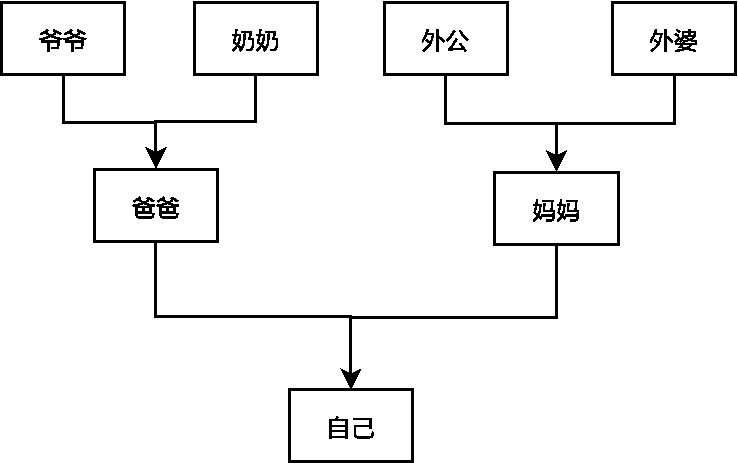
\includegraphics[keepaspectratio,max width=0.95\linewidth]{figures/亲属关系.png}
\caption{亲属关系}
\end{figure}

据《圣经》记载,今天地球上所有的人类都是有一男一女生出来的,那个男的名叫亚当,那个女的名叫夏娃。且不管这是真的还是假的,遗传学家史宾赛·韦尔斯(Spencer Wells)通过Y染色体分析似乎找到了“亚当”存在的证据,这里更确切的表述是至少确认在6万年之前Y染色体发生了一个变异,我们今天地球上所有的男人的Y染色体上都能找到这个变异,简单来说就是确认在六万年之前有那么一群亚当(甚至一个亚当)是现在所有男人的祖先。而有意思的是科学家们从线粒体上的基因序列进行分析似乎也得出了类似的“线粒体夏娃”的概念,不过关于这样一群亚当和夏娃(或者正如《圣经》所言只是一对)究竟从历史上什么时候开始出现科学家们还存在很大的争议,但我想人们对于这样一个概念已经有所共识了:那就是今天我们所有的人类都来自一小群原始人。

那么用图画表示这样的过程是怎样的呢?\footnote{我们且先不论近亲繁殖。。}

\begin{figure}[H]
\centering
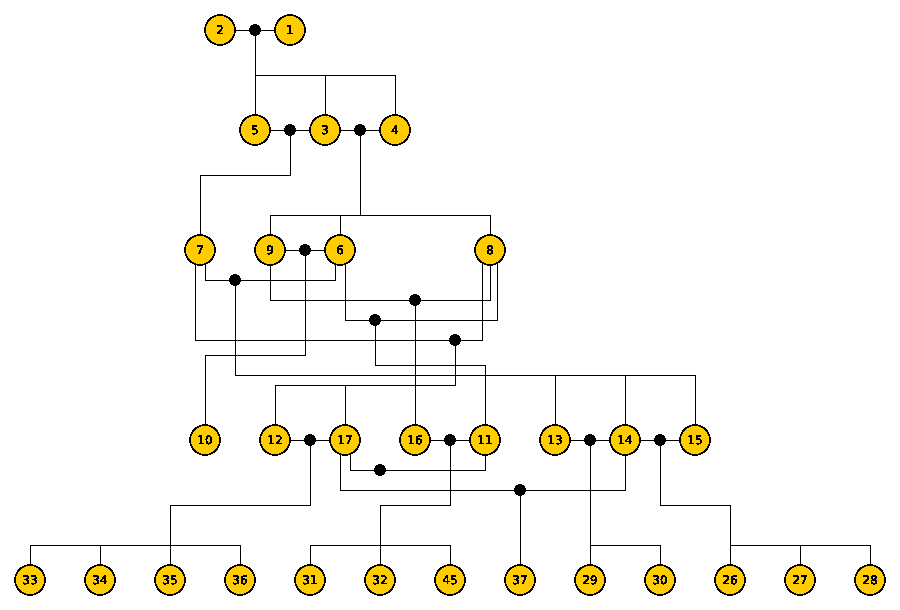
\includegraphics[keepaspectratio,max width=0.95\linewidth]{figures/族谱图样.png}
\caption{族谱图样}
\end{figure}


\section{生活大爆炸}
\label{sec-2}

目前的科学认为(科学总要讲证据的,他们这样认为肯定有相应的证据,至于具体事实是不是这样那就另当别论了)我们的这个宇宙源于一个非常非常小的奇点,奇点将整个宇宙的物质甚至是空间和时间都聚集在了一起,也就是这个奇点的外面不仅没有什么东西,而且连空间和时间都没有。然后不知道怎么的,(这之前的细节科学家目前也不清楚)宇宙大爆炸了。大爆炸理论的第一个弱证据是哈勃定律说明了宇宙在膨胀(宇宙在膨胀人们可以反向想到可能之前的宇宙很小很小),大爆炸理论最直接和最重要的一个证据是宇宙的微波背景辐射的发现,这个发现使绝大多数物理学家都相信宇宙起源于一次大爆炸。

关于大爆炸理论最新的进展是2014年科学家们宣布观测到了引力波,这为暴胀理论提供了重要的证据。暴胀理论认为大爆炸刚开始存在一个暴胀阶段,也就是宇宙迅速的膨胀,膨胀速度远超过光速,暴胀之后宇宙还在继续膨胀,不过速度慢的多了。科学家们观测到的引力波可能就是这一次暴胀产生的猛烈的冲击才出现,而暴胀理论为宇宙的各向同性和微波背景辐射的均匀分布都提供了良好的解释。

\subsection{时间和空间}
\label{sec-2-1}
\begin{quote}
起初,神创造天地。
地是空虚混沌,渊面黑暗,神的灵运行在水面上。 
\end{quote}


如果我们要上演一出戏剧,那么首先要搭好舞台,这个舞台之于物理学就是时间和空间。如果暴胀理论是正确的,那么到底什么东西跑得这么快呢?我假设就是时间和空间吧,那个时候光子都还没生成出来,所以到处是一片漆黑,而奇点聚集的物质也许就是圣经里面所说的水面吧—— 一切能量的源泉。


\subsection{光}
\label{sec-2-2}
\begin{quote}
神说:要有光,就有了光。 
\end{quote}


目前物理学观测的粒子都没有打破光速不变且不可超越的定律,是不是从观测上必然观测不到超光速的存在这个我不大确切。但是光(电磁波)作为我们已知跑得最快的物体,是继时间和空间之后第二个跑出的东西似乎还是有些道理的,想像一下吧,奇点的吸引力多么的强,当然是跑得最快先跑出来了。


\subsection{各种各样的粒子}
\label{sec-2-3}
\begin{quote}
神说:诸水之间要有空气,将水分为上下。 
\end{quote}

随着宇宙的膨胀和冷却,开始出现越来越多的细小粒子,我们可以想像刚开始,可能出现的很多粒子结构都不太稳定,寿命很短。而只有那些结构优化了的,寿命较长的粒子慢慢积累了起来(粒子的进化史)。于是就有了我们常常听到的名字,夸克,胶子,质子,中子,电子或者什么什么子。同时还有大量的反物质,比如反电子,反质子,或者暗物质等等?

终于宇宙中到处都是氢气(一个质子和一个电子组成)了。而接下来大爆炸理论迎来了预测最成功的部分——太初核合成,也就是大爆炸后第3分钟到第20分钟。那个时候原宇宙进行了十几分钟的核合成反应。就是这短短十几分钟的核合成反应,构成了我们这个宇宙的一般元素丰度比(越古老的星云越接近这个比值)。因为太初核合成只进行了短短十几分钟,然后原宇宙温度就下降到不足以发生核聚变了,所以宇宙元素丰度大部分都是氢原子,然后有少量的氦原子和极少量的氘原子(一个质子一个中子一个电子),然后还有几乎可以忽略不计的微量锂原子,后面的重元素就可以视为没有了。

随着粒子的相互作用,它们就形成了我们今天看到的星云,这只是它们庞大成员中的一个例子:

\begin{figure}[H]
\centering
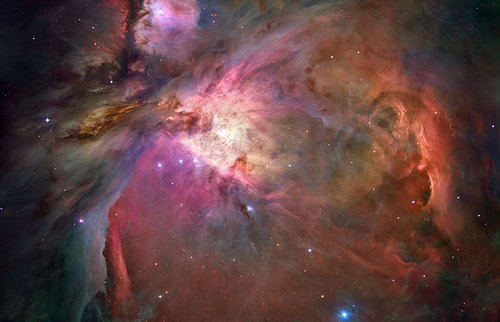
\includegraphics[keepaspectratio,max width=0.95\linewidth]{figures/星云.jpg}
\caption{星云}
\end{figure}


\section{宇宙}
\label{sec-3}
下面图片中这个花瓣形状的图案在印度文化中名字叫做mandala(曼荼(tú)罗),它代表着宇宙的模型。这个图形符号有很多变种:

\begin{figure}[H]
\centering
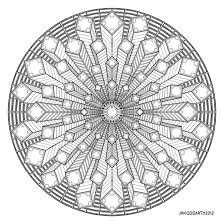
\includegraphics[keepaspectratio,max width=0.95\linewidth]{figures/mandala-1.png}
\caption{mandala-1}
\end{figure}
\begin{figure}[H]
\centering

\includegraphics[keepaspectratio,max width=0.95\linewidth]{figures/mandala-2.png}
\caption{mandala-2}
\end{figure}
\begin{figure}[H]
\centering

\includegraphics[keepaspectratio,max width=0.95\linewidth]{figures/mandala-3.png}
\caption{mandala-3}
\end{figure}


这些图形的相似之处就是有很多类似的元素(图形子单元)绕着某个中心以漩涡的形式向外扩散。而这种扩散的漩涡和向日葵和银河系的图案都有某种相似之处:
\begin{figure}[H]
\centering
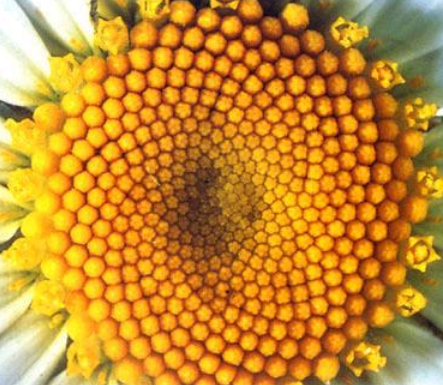
\includegraphics[keepaspectratio,max width=0.95\linewidth]{figures/向日葵.png}
\caption{向日葵}
\end{figure}

\begin{figure}[H]
\centering
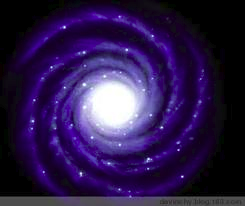
\includegraphics[keepaspectratio,max width=0.95\linewidth]{figures/银河系.png}
\caption{银河系}
\end{figure}

上面第二张图就是我们的银河系,而我们的太阳系就在银河系边缘的一个角落里安静地绕着银河系中心旋转着。我不能将不同形状的星系图片在这里列出来,但是我执意要将我们这个宇宙有多少个星系(银河系在漩涡星系里面属于中等个子)的大概数字列出来,是11个零:100 000 000 000。而银河系里面大约也有11个零的恒星(太阳就在其中),那么宇宙中大约有11个零乘以11个零的恒星数目,即大约有10 000 000 000 000 000 000 000 000 000 000 000 000 000 000 000 000 000 000 000 000 000 000 000 000 000 000 000 000 000 000 000 000 000 000 000 000 000 000 000 000个恒星。宇宙是如此的巨大 ,是不是只有银河系里面的太阳系里面的地球才有可能有生命呢?

\subsection{六日创世}
\label{sec-3-1}
\begin{quote}
神看着一切所造的都甚好,有晚上、有早晨、是第六日。 
\end{quote}


\begin{table}[H]
\caption{六日创世时间表}
\centering
\begin{tabular}{p{0.18\linewidth}|p{0.72\linewidth}}
\toprule
时间(亿年前) & 事件\\
\midrule
137-115 & 第一日:大爆炸和太初核合成等创造各种基本粒子,基本奠定了目前宇宙的时间空间和星系分布情况。\\
115-92 & 第二日:各大星系衍化发展,超新星核合成制造出重元素,为第一批行星的出现做准备。\\
92-69 & 第三日:第一代行星形成,并进化出了第一代生命形式,那个时候生命形式比较单调,除了最简单的生命形式外,似乎植物的各个类别都进化出来了。\\
69-46 & 第四日:第二代星系(如太阳系)出现,第二代行星形成,太阳地球月亮基本运行情况确立。\\
46-23 & 第五日:第二代星系的特点可能是重元素含量更高,它进化出了第二代生命形式(第二代生命形式可能基于第一代生命形式,也可能不同,只是后来发生了融合),也就是各种各样的水里的动物。\\
23- & 第六日:正如生物课所讲述的,氧气出现,动物植物登陆,两栖动物,爬行动物,哺乳动物直到人类出现等等。\\
\bottomrule
\end{tabular}
\end{table}


现代科学认为大爆炸距今137亿年,如果按照《圣经》所说是六日创世,那么一日就是23亿年。如是对照圣经我建立了这样的时间表。

\subsection{我的辩解}
\label{sec-3-2}
\subsubsection{重元素生成}
\label{sec-3-2-1}
之前我们提到过太初核合成时间太短是不能产生重元素的,这就造成了一个问题,因为我们地球就是一个重元素行星,也就是说地球上所有的重元素都不是太阳造的,太阳只是将这些重元素捕获罢了。这告诉我们一个简单的事实(假设星系之间物质基本没有什么交流了),那就是太阳系至少是继第一批超新星爆炸之后才形成的(现在科学认为宇宙中的重元素主要由超新星核合成而来。)

\subsubsection{进化加速现象}
\label{sec-3-2-2}
虽然达尔文的进化论思想深入人心,人们也愿意相信地球是一个生命形式的原创者。但是随着现代科学的进步,人们对细胞以及各个生物的器官构造了解的深入,尤其是对DNA分子里面承载着整个地球的巨大的生物信息量,使得人们总感到进化论就靠简单的自然选择和随机突变就能进化出如此完美多样的生物形式,这一说法太过于难以让人们无法相信。就好比现代物理学中量子理论那样要别人相信,一个猴子就是在打印机上随机随便乱打也能打出莎士比亚的作品,然后人们选择出那个好的作品就可以,这太过于不合情理。

其实我内心深深相信这样一个神秘的观点,宇宙具有比我们更高级的智慧,如果我们都懂得不能同一个地方多次摔跤几次,如果找到事物好的解决办法那么下次就应该参考这个,那么难道宇宙就这么蠢,不懂得这些吗?所以我相信不管是粒子的进化还是生物的进化,整个宇宙存在着一种信息共享机制。

但是作为我保守的表面,在面对宇宙信息的累积现象和生物的进化加速现象时,还是让我这样说吧,地球的DNA信息来源可能不是独创,可能地球上的所有生物都是在第一代行星上繁衍出的第一代生命形式的基础上进展下来的。至于具体通过何种形式,是细菌还是病毒藏在岩石里面传播的,甚至是某种高等智慧生命传播的,那就不得而知了。


\section{太阳系}
\label{sec-4}
\begin{quote}
神说:天上要有光体, 可以分昼夜、作记号、定节令、日子、年岁。
于是,神造了两个大光,大的管昼、小的管夜。又造众星。  
\end{quote}

太阳系各大行星具体是如何运行的牛顿时代就能够算得很清楚了,不过牛顿一直对各大行星是如何获得这个第一推动力让它们绕着太阳转这个问题耿耿于怀。那是因为他没有想到太阳系也有一个形成的过程,而且那个时候的太阳系可不是这么风平浪静,时不时的有小行星撞了进来。目前有的科学家认为月亮是撞出来的,有的科学家认为地球上的水也是小行星带过来的,所以有的科学家认为地球上的生命形式也是小行星带过来的也不足为奇了。总之关于太阳系早期的历史具体发生了还有很多未解之谜等着各位去探索。

不管怎么样在大约46亿年前的时候,地球月亮和太阳系已经基本成型了,那个时候地球上虽然表面很烫,时不时有火山喷发,但也是有白天和晚上了,而且到晚上也开始有很多星星在闪烁了(星星都是恒星,行星是看不见的。)地球的寿命是通过一种同位素的衰变规律测定的,可信度还是很高了。


\section{生命的起源}
\label{sec-5}
\begin{quote}
神说:水要多多滋生有生命的物,要有雀鸟飞在地面以上、天空之中。  
\end{quote}


\subsection{生命之光}
\label{sec-5-1}
宇宙存在着一种力量,这股力量就是时间。时间就好像一把筛子,把结构稳定的粒子留了下来。而生命不同于非生命的最大区别就是他们对抗时间的方式不是因为自身的结构多么牢不可破,而是他们身上的信息可以复制下去,生命通过复制自己来对抗时间。我只能猜测生命之光的产生的内在推动力不是自然选择,说自然选择能够作用于非生命实在荒唐,也不是时间,时间和自然选择一样只是一种被动的力量。我们还需要一种力量,这股力量就是作用于各大基本粒子的力量,让他们不断产生出最新形式的粒子,我也相信正是这股力量产生了生命之光。

生命之光和其他非生命最大的本质区别就在于他能够复制自己,人们现在似乎相信RNA就是那一道生命之光,可是RNA在我看来还是太过于复杂,我相信那一道生命之光就存在于化学的世界里。

\subsubsection{分子的世界}
\label{sec-5-1-1}
在第一代行星的上面,那里就已经有了丰富的铁上面(元素周期表之前)元素。这些原子不断和其他原子发生着化合反应。其中碳原子和其他原子构成的形式多样的有机化合物格外引人注目,下面这张图是常见的元素周期表。

\begin{figure}[H]
\centering
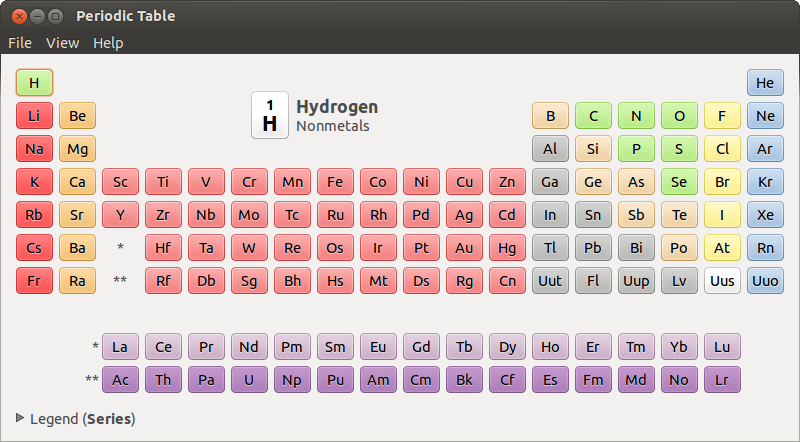
\includegraphics[keepaspectratio,max width=0.95\linewidth]{figures/元素周期表.png}
\caption{元素周期表}
\end{figure}


我相信就是从氢原子到铁原子中某一种形式的有机化合物在某种环境下可能具有了生命的特征,那就是能够复制自己,而在其他环境下则跟一般的非生命物质一样,这就是第一道生命之光。而后面所有的生命都是在这第一道生命之光的基础上发展出来的。关于谁是这一道生命之光,有的科学家认为是DNA,有的认为是RNA,也有的认为是蛋白质,这个也是一个极有争议的问题。


\subsection{水是关键}
\label{sec-5-2}
正如前面提及的,地球上的生命首先都是生活在水里面的,所以生命的起源首先面对的一个问题是水的起源。

太阳系基本成型之后,小行星撞击地球的几率开始变小了,因为木星等行星正在为地球保驾护航。没有小行星撞击带来的巨大的热量,地球运行的轨道开始变得稳定,地球的表面也开始冷却,然后水蒸汽慢慢降了下来,然后就开始下雨了,下了几天几夜的雨啊!雨下着下着就有海洋了。

这些水蒸汽的来源还是一个很有争议的问题,这个时候人们会想到会不会存在这样一个时期,在地球表面冷却到雨下下来,那样一个短暂的时期,地球上所有的水都以水蒸汽的形式就好像云一样,水滴里面含有的物质更杂。嗯,这就好像米勒-尤里实验所模拟的那样,不同的是这里认为“米勒-尤里反应”主要发生下雨之前,因为那个时候空气中水分含量更加充足,这样将形成一层所谓的水蒸汽大气层,这层水蒸汽大气层是如此之厚,想象一下当时地球上所有的水都漂浮在上面的。所以在这么厚的一层水蒸汽大气层上发生的化学反应可能分为(按照海拔高度)好几个层次!第一个层次可能是类似米勒-尤里实验演示的有基本的氨基酸和其他小有机分子生成;这些基本的氨基酸分子和其他小有机分子沉降下来,然后是第二个层次等等,具体过程可能很复杂,但我知道在最下面的层次里面可能紫外线干扰已经不存在了,其次可能有其他火山喷发的无机物质加入进来漂浮其中进行了某些必要的化学催化反应和化学合成反应,其次水分子在不同温度不同压力下的漂浮形态也是值得我们思考的一个问题。

那么是不是由这样更加复杂的米勒-尤里反应产生了第一道生命之光,甚至是更加复杂结构的生命形式?我看很有可能。所以故事发展到现在,地球开始下雨了,下的是有机雨。这样的有机雨构成了早期的海洋,可以想象早期海洋有机质含量非常的高,然后随着下雨的进行有机质含量开始变低了,正是这样的环境构成了地球上生命的摇篮。

地球的表面虽然冷却下来了,但是地球的内部岩浆还是很热很热的,时不时的有火山喷发和推动板块漂移,这些对生物的进化也可能起了很重要的作用。



\subsection{各种各样的生命}
\label{sec-5-3}
细胞就是生物界的“原子”,而且是以一种更加复杂的形式。 当我们看到细胞具有如此复杂巧妙的结构和内部有如此丰富的内容时,我的第一反应是争论第一道生命之光可能没有意义,细胞是一个组合体,那么他体内的每一个自身部分的复制可能之前都有了相应的存在。比如线粒体,叶绿体,核糖体,高尔基体,溶酶体,中心体等等。他们是细胞的构成单元,也就意味着在细胞之前这些东西可能都已经存在了,而且都已经存在着对应的复制机制,细胞就是将他们的复制机制融合在了一起。他们就好像一堆子程序,然后融合在了一起成了一个更强大的程序,而且因为他们都共享一套基因信息编码规则,使得他们融合起来应该难度不大。

在那场有机雨里面生命的结构形式已经复杂到了何种程度不得而知,正如之前所述地球可能并不是一个生命形式的原创者或者只是一个部分创新者,所以不敢保证那场有机雨里面是不是已经有了外来的DNA或者什么信息。保守起见我们可以这样说,那场有机雨里面至少已经有了某些复杂的蛋白质,可能简单的DNA或者RNA等复杂有机分子也已经少量含有了。

接下来海洋的温度慢慢冷却,海洋里面的有机质浓度随着下雨慢慢冲淡,前面叙说的生命之光,某些具有自我复制能力的小有机分子(可能某些蛋白质某些小片段DNA)开始在时间的作用下大发神威,繁衍改造着周围的有机质(这个时候细胞的构成单元比如线粒体,核糖体附带自己的DNA信息可能都已经存在了。)米勒-尤里反应可能差不多已经停止了,我在这里再强调一次有机质浓度变淡这个事实,在地球海洋有机质浓度变淡到一定程度的时候,生命具有移动能力就变得非常重要,我只能说大概在某个点上,原始的具有移动能力的更加复杂一点的生命形式开始大量繁衍了\footnote{只能说开始大量繁衍了,不能说开始出现了。}(这个时候进化论的自然选择学说开始发挥作用了)。在“野外”有机质浓度进一步降低甚至可以视为没有的时候,原始的植物代表(吸收光能\footnote{或者其他能量?}制造有机质),原始的动物代表(吞噬别的生命来获得有机质)开始大量繁衍了。


\section{进化论}
\label{sec-6}
\begin{quote}
神就赐福给这一切,说:滋生繁多,充满海中的水。雀鸟也要多生在地上。 
\end{quote}


接下来就是为大家熟知的进化论部分,从细胞开始,变异,自然选择,进化。从单细胞到多细胞,从无脊椎动物到脊椎动物直到出现鱼类。唯一不懂的就是为什么《圣经》要提及雀鸟。且不管这个吧。

这一块涉及到的生物学知识杂而多,实际上很难说那一次变异具有革命性意义,哪一种功能的出现会让这种生物获得核心竞争力。所以我一笔带过,只是简单地说到接下来是进化论的研究领域,那里天天发生生物改变环境或者被环境改变和生物之间相互改变的故事。


\subsection{登陆!}
\label{sec-6-1}
\begin{quote}
神说:地要生出活物来,各从其类。牲畜、昆虫、野兽、各从其类,事就这样成了。 
\end{quote}


生物登陆是人们回顾地球历史最喜欢谈及的一个事件,因为它首先表现效果明显,改变了地球大陆的模样;其次它和一个核心事件那就是氧气浓度的升高和臭氧层的出现相关;最后从人类的进化角度来说它意义非凡。

氧气的出现对地球生态圈上的生命产生了重大的影响,可以说是再造了整个生命界,我生物学方面不大精通,这里略过。重点谈一谈脊椎动物从鱼类到两栖类到爬行类到哺乳类的进化路线。这一条路线最显著的一个特点就是神经系统和大脑变得越来越发达,我以为从登陆后地貌的多变,气候的多变造成的环境的多变对脊椎动物的大脑进化主路线起了重要的作用。当然了还有很多器官很多功能的进化都是为了适应陆地上环境的多变的,比如人们现在普遍相信恐龙灭绝与一次小行星撞击事件造成的环境的剧烈变化,从而哺乳类开始崛起。不过就算地球不发生那次巨大的小行星撞击事件,也难说恐龙后面会竞争得过哺乳动物。


\subsection{从信息看进化}
\label{sec-6-2}
宇宙在时间的演变中不断发展出新的信息载体, 从信息的角度来看,实在没有大小之分,从信息量来分析宇宙这些年所走过的道路总能带给人们一些启迪。

\begin{description}
\item[{物理粒子}] 如果弦论所述是真的话,那么粒子的信息主要是特定形式的共振波保存着的。
\item[{化学分子}] 化学分子严格意义上讲也可以视作一种更复杂形式的波,但我们说它主要是以不同原子的不同构造形式保存的。
\item[{生命}] 生命以一种非常复杂的化学分子DNA作为载体保存信息的,DNA里面的信息可以简单视作“0”和“1”二进制的编码。
\end{description}


生命的所有信息不是都存储在DNA分子里面的,接下来的描述也许有些人不信,但也许很有价值。下面我要描述大脑的四个进化阶段:

\begin{itemize}
\item 神经系统所含信息超过基因信息,代表着个体的生存对基因的传承也很重要,不一定只是简单的多生育即可。我以为这个关键点大概在爬行动物那里。我把爬行动物进化出来的大脑叫做本能脑,意思只是简单对外界环境进行本能式的反应。
\item 大脑中的皮层脑信息超过了本能脑所含的信息,代表着基于现在环境的判断从而做出反应比简单的过去传承下来的程序式反应更能适应环境。我以为这个关键点大概在哺乳动物那里。我把哺乳动物进化出来的大脑叫做皮层脑,皮层脑和视觉触觉等身体上各种感官器官发生着联系,并不断记录这些信息从而做出分析和判断。
\item 大脑中的额脑信息超过皮层脑信息,额脑是大脑中很奇特的一个结构,值得大讲特讲,不过这里只是简单提一下。原始人类比如说直立人他们早期只进化皮层脑,这个时候他们实际上还算不上人类,只能算是一种特殊的哺乳动物,真正意义上的人类的出现是智人,我将那一批进化到我们现代人的智人称为原人,那么这些原人最大的特点就是他们的额脑。额脑是大脑的一个什么东西,它没有和任何感官器官相联系,只是广泛地和皮层脑发生联系,其结果就是抽象思维,宗教的萌芽等等都出现了。简单来说就是原人不是一个只活在由皮层脑构造出来的信息世界里,他们还活在由额脑构造出来的理念世界里,借助这个理念世界,第一次生物具有了通过想象力改造世界的能力,他们对未来开始有了一定的概念,可能开始隐约体察死亡的存在了。那么额脑的好处何在呢?好处就是原人已经具有了初步的根据目的制定计划的能力。关于这方面还可以说上很多,尤其是额脑如何控制皮层脑的随机漫游(做梦)主动虚构信息,主动创造信息等等。这里略过了。
\item 社会传承的信息超过个体大脑的信息,原人也有一定的社群,但他们可能还没有文化传承。目前考古发现的智人大约出现在20万年前,那么第一批原人是不是就是本文刚开始我提到“亚当”和“夏娃”呢?这不得而知,不过我们知道的是原人慢慢开始发展出了自己的语言(其实动物也有简单的语言和简单的使用工具的能力)和自己的工具,并且有了宗教和对生死的思考,然后早期他们的文化传承就通过宗教的形式进行下去的。于是新的石器,新的狩猎方式等等使得原人迅速崛起遍布全球,形成了今天的万物的灵长——人类。人类是一个年轻的物种,能够如此短的时间内迅速崛起不得不承认这是一个极具戏剧性的事件。
\end{itemize}




\section{人类文明}
\label{sec-7}
在提及人类这个物种的时候,就不得不提到文明这两个字,因为单个人类进入大自然的生存斗争,既无庞大的体形,也无锋利的爪子和强健的体魄,如果瘦弱不堪的一个物种很难和他目前取得的成就相提并论。

同时在提及人类文明的时候又不得不再一次强调这个事实,所谓文明的根基就是代代传承工业技术和政治文化。人们对工业技术的传承看得很清楚,石器时代,陶器时代,青铜器时代,铁器时代,现代工业等等,但是人们对政治制度的传承的重视程度总是不够。比如我现在把你放入亚当夏娃时代,那么时候你遍地的石头你如何利用你现在脑子掌握的各种高端科学技术?最后你还是要从打磨石头开始,但有一种东西你可以和你的族群分享并让他们得到实实在在的好处,那就是政治文化。比如你可以教他们团结,学会合作解决问题,教他们学会合作狩猎共同抵御外敌等等。这正是我要提出的人类文明的关键变革点不是由工业技术的变革决定的, 而是由政治文化的变革决定的。因为工业技术它有自身的积累规律,到了一定阶段必然发生突破,而政治文化带有更大的自由性。

现在我按照政治文化的发展阶段叙述人类文明:
\subsection{部落文明}
\label{sec-7-1}
原人早期是部落文明,部落文明最大的特点就是人们从事狩猎采集活动,一般十几个人组成一个小部落,如果人数多了他们中的某一支就会分离迁徙,因为就狩猎采集来说实在没必要要那么多人,人多了他们就会吵架,因为肉分得不均匀,肯定是参加狩猎的那部分人肉分得多些。然后早期并没有什么首领的概念,就是家长,家长负责传承知识之类的。所以一个部落就好像一个小家庭,但这并不意味着他们内部没有冲突很和谐,可能平时矛盾绝不在少数,而他们解决矛盾的方式很简单,判决谁谁谁分离迁徙出去。

\subsection{大部落文明}
\label{sec-7-2}
具体这种转变是怎么发生的不太清楚,不过从目前看来地球各地人类文明来看,还是有一些地方的文明一直停留在狩猎采集(我将捕鱼也归为采集)活动阶段,如果你们认为他们蠢发展不出更新的技术我严重怀疑这一点。那么为什么他们一直停留在部落文明阶段而不是走向大部落,发生部落的融合呢?我的解释是他们的人口没有扩大到一定数目。

再来说一下那些发生大部落文明的地方,他们有两种部落沟通的方法:第一种是认为别的部落都是和他们抢粮食的,都是坏的,这就是他们的政治文化,这些部落(比如食人部落)大多发展不起来,几乎快灭绝了;第二种是认为别的部落也是人,也应该和他们一起合作。这种合作的具体形式就是交易,其实婚姻也是一种交易。

几个部落交易之后因为交易要有守则,要大家都懂规矩,于是道德出来了。人类道德的核心价值离不开交易二字。然后道德审判的大祭司啊酋长啊首领也被大家选举出来了,然后宗教进一步发展出来,整个大部落文明形成了以宗教为中心的教育,艺术等等。

几个部落发生交易之后,经济学的分工概念出来了,然后人们会自觉去寻找那些他们产量最高的行当,这样整个大部落都获得了最大利益,然后都变得更强了。早期的分工可能还是只有采集,狩猎和制造简单石器等。那么那些狩猎采集等能力差的会怎么样呢?这个时候他不是要迁徙或者对抗,而是选择另辟蹊径,我相信大部落文明中期的时候分工大致有了:采集,狩猎,制陶,畜牧等,而到了大部落文明晚期开始出现农业了,而且随着采集,狩猎行业的衰落,农业部落的崛起,这个时候人类文明就要开始进入国家文明阶段了。

\subsection{国家文明}
\label{sec-7-3}
原有的采集狩猎行业都要衰落下去,而农业行业继而发展之。这个时候采集狩猎的部落要某转型为畜牧要某就转型为这个部落的守卫力量。因为恰好农业这个行当对地皮的需求是极其强烈的,而这极容易和其他部落发生冲突,这个部落的守卫起初只是内部协调部落间的冲突,然后国家的长官也选出来了(可能就是之前的大祭司酋长首领转型过来的,也可能不是。)然后国家文明的社会规则法律也出现了。

接下来的事情大家历史学得比我好,我就不多说了。值得一提的是在国家文明大框架下,后面农业文明和畜牧文明发生了极大的冲突,如前所述,狩猎部落转型为畜牧,所以他们大多彪悍;而原狩猎部落转型为部落守卫力量的多少有点养尊处优。很难说这场农业文明对抗畜牧文明的战争谁赢谁输。

目前我们人类的文明还是处于国家文明阶段, 农业文明和畜牧文明的冲突从某种意义上还在继续着,同时各个国家之间冲突也在继续着,而国家对于地皮争夺的狂热也还在这个世界的人们心中延续着(因为人们从地皮之上又发现了新的资源),不管是中国还是现在美国,不管是专制的国家还是所谓的民主的国家,他们似乎内心都对面积庞大的帝国抱有一丝赞叹和羡慕之情。

如前所述,促使人类文明从部落文明过渡到大部落文明的是交易精神,而促使大部落文明过渡到国家文明的是什么精神是什么政治文化呢?我发现我对这个问题还没找到答案,也许在座的各位有了一些想法。也许国家文明的本质就是基于地皮的武装对抗,也许将来世界上所有的国家都将消失而回归到基于交易的大部落文明,或者由国家文明进化为另一个新的文明阶段?

人们总是在赞叹文艺复兴和近代科技的进步,作为科技进步的加速现象这是好理解的,同时人们看得更加清楚的是没有文艺复兴,没有欧洲的这一场政治文化革新,可能后面的所有科技进步都将化为泡影或者无限期推后。有人问为什么其他地方科技没有进步,其实他们应该问为什么其他地方没有发生文艺复兴。那么文艺复兴意味着什么,是一个新的全人类的文明阶段吗?我不敢断言。



\section{未来或者总结}
\label{sec-8}
宇宙经历了怎样的旅程才生出这样一个你呵!那么我要怎么描述今天这个时代?是科技快速进步的时代吗?不!我要告诉你,我们处在国家文明的晚期,我要告诉你们我们还处在文艺复兴时期,我要告诉你,人,就是你自己,才是这个世界上最宝贵的财富。

那么人类文明的未来如何呢?是被机器人文明取代,还是走向星际文明,还是文明终结。谁知道呢?走过了这一程,这一路不易,但绝不是不可复制。这一路走来到处充满了奇迹和偶然,甚至也许宇宙中只有地球才有人类这样的智慧生物也是可能的,但这绝不意味着人类的未来就拴上了安全保险。如果上帝创造了宇宙,通过种种造化神功生出了人类,那么没有任何理由可以怀疑上帝没有能力再造一个。

抛开宗教和神秘主义不谈,最后让我再问一次,宇宙的终极目的何在?我发现我脑子里浮现出好多神秘主义的猜测,有佛教宇宙如是泡影,有多态平行宇宙等等。这些不能带给我半点思想上的教益,于是我把这些都统统抛弃了,就如同我追寻生命的意义一样, 我给自己这样答道: \uline{我是宇宙的一部分,所以让我用自己的头脑思考宇宙,认识宇宙,活出宇宙的意义出来吧} 。



\section{参考资料}
\label{sec-9}
\begin{itemize}
\item google图片搜索——mandala,银河系。\href{http://amuseum.cdstm.cn/AMuseum/math/6/608/6_608_1002.htm}{向日葵}。
\item 维基百科:Y染色体亚当,大爆炸,引力波,宇宙暴胀,太初核合成,星系,超新星核合成,地球历史,细胞,米勒-尤里实验。
\item \href{http://bible.kuanye.net/hhb/}{圣经参考网站}
\end{itemize}
% 编者:万泽
\end{document}